\\
ERC is a complex endeavour that includes not only comprehending the intent and context of a conversation but also the capability to model the emotional modulation between speakers, taking into consideration the inter and self-speaker influences [3]. Furthermore, the task is hampered by the scarcity of annotated data, particularly in multimodal instances, and variances that arise as a result of the subjectivity of annotators in understanding emotions [4]. 

To tackle these challenges, Hazarika et. al. created the \textit{TL-ERC} paradigm, which employed sequential inductive transfer learning. The purpose was to use contextual affective information from a generative conversation modelling system to recognise emotions in natural conversations \cite{Hazarika2019ConversationalTL}. The novelty in their approach was to investigate and reason why generative models would see fit to gather insights about emotional dynamics. They used prior works to establish that emotional objectives and impacts worked as latent drivers in dialogues. The interconnectedness of numerous factors, such as the theme of the conversation, temperament of the speaker, their logical thought process, perspective and motivation, were responsible for altering their emotional state, eventually resulting in an utterance \cite{Weigand+1998+35+48, Poria2019EmotionRI}. The authors used example Fig \ref{emotional_dynamics} to demonstrate such inconspicuous emotional dynamics that organically craft conversations. In light of this, they speculated that since an ideal dialogue generator would need to decipher hidden emotions from the contextual settings of their historical utterances and characterise the trajectories underlying them, they might be able to depict implicit affective patterns throughout a conversation \cite{Shimizu2018PretrainingSC}. In order to transfer this knowledge into their intended discriminative task, namely ERC, they offered a strategy that employed transfer learning.

\begin{figure}[ht]
\centering
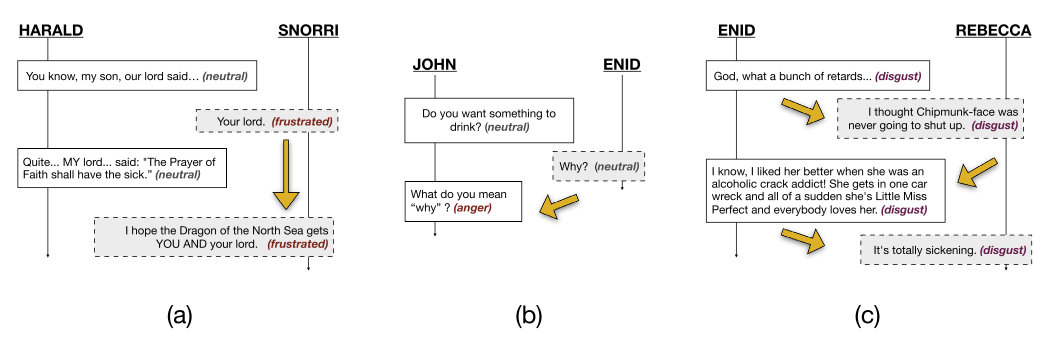
\includegraphics[width=0.9\textwidth]{Figures/Fig1-5.png}
\captionsetup{justification=centering}
\caption{Hazarika et. al. \cite{Hazarika2019ConversationalTL} -- Illustrations for the concepts of (a) \textit{emotional inertia} or self-influences in emotional states \cite{Koval2012ChangingED}, (b) \textit{emotional transitions} or \textit{shifts} due to external influences, and (c) \textit{mirroring} or topical agreement between speakers \cite{Navarretta2016MirroringFE}}
 \label{emotional_dynamics}
\end{figure}

The authors proposed to pre-train a hierarchical generative dialogue model on the \textit{source} task of conversation modelling as this unsupervised or self-supervised activity usually gained from a significant amount of data in the form of multi-turn dialogues. After pre-training, the model was fitted to the \textit{target} task of ERC by transferring the inter-sentence contextual parameters from the trained source model. To encode sentences, they used BERT \cite{Devlin2019BERTPO}, that is trained to meet concealed language modelling and next sentence prediction goals.

For the source task of generative conversation modelling, the authors used the Hierarchical Recurrent Encoder-Decoder (HRED), a traditional framework for seq2seq conversation answer generation that analyses conversations in a systematic order \cite{Serban2015BuildingED}, with three serial elements -- an encoder RNN for paired sentence and preceding context encoding, a context RNN for explicitly modelling the conversational context spanning utterances up until the current time-step $t$, and an auto-regressive decoder RNN for generating the response statement conditioned on the collective encoded context. Each conversation $C_i$ was considered as a collection of sequential utterances $[x_i,_1,...,x_i,_{n_i}]$. The HRED trained all conversations $C_i \in C$ in the dataset cumulatively by using the maximum likelihood estimate criterion $arg\,max_\theta = \sum log\,p_\theta(C_i)$. The authors used the original version of the HRED model architecture with single-layer components in order to keep the hypothesis simple and avoid the extra complexities of multi-layer RNNs and other novel encoding techniques provided by them. They modelled the encoder function of the sentence encoding RNN using a bi-directional Gated Recurrent Unit (GRU) \cite{Cho2014LearningPR} and used its uni-directional variant for the context encoder and decoder, while supplementing the decoder with a beam-decoding functionality as done by \cite{beam-decoding}.

 The infrastructural setup for the target task was similar to that of the source domain, as carried out by \cite{poria-etal-2017-context}, with the exception of the decoder being replaced by a discriminative mapping to the label space for classifying the emotion. The input to this model was a conversation $C$ with member utterances $[x_1,...,x_n]$ with each $x_i$ having an associated emotion label $y_i \in Y$. Hazarika et. al. utilised BERT \cite{Devlin2019BERTPO} to model utterances for the target task and expressed its parameters as $\theta^{BERT}$ (obtained from the source model - $\theta^{source}_{enc}$), only keeping the first four layers of the model to prevent parameter explosion. The hidden vectors of the $[CLS]$ token across were mean-pooled across the studied layers to obtain a sentence representation. They chose BERT as it outperformed the HRED sentence-encoder in terms of encoding power and inter-sentence level abstraction. The learned parameters of the GRU function of the context encoder in the source model were retained and transferred while an additional set of new weight and bias parameters were introduced for the dense layers in the target model, thereby leading to a final parametric representation $\theta^{source}_{cxt}$. The training of the classification layer was done using the cross-entropy loss and its output was the projection of the context RNN onto the label embedding space.

 Hazarika et. al. used the Cornell movie \cite{DanescuNiculescuMizil2011ChameleonsII} and Ubuntu dialog \cite{Lowe2015TheUD} corpora, two vast dyadic, bi-party conversational archetype datasets, to train their models for the conversation generation task. The dataset partitions were developed as recommended in \cite{Park2018AHL}. For the target task, they used the text mode of the small-sized dataset IEMOCAP, which consists of dyadic conversations between 10 speakers and emotion labels for \textit{anger, happiness, sadness, neutral, excitement}, and \textit{frustration}; the medium-sized chat-based dataset DailyDialog with emotion labels for \textit{anger, happiness, sadness, surprise, fear, disgust} and \textit{no\_emotion} \cite{Li2017DailyDialogAM}; and the regression-based dataset SEMAINE, a video-based corpus of human-agent emotional inflections \cite{5959155}. The dataset's emotional labels are \textit{valence, arousal, power} and \textit{expectation}, and the annotations were set up to be aligned with \cite{hazarika-etal-2018-icon}. 
 
 The DailyDialog dataset was very lopsided, in contrast to the well-balanced IEMOCAP dataset. The authors used the weighted F-score to evaluate these two datasets. However, the \textit{no\_emotion} class in the DailyDialog dataset had the most instances with 82.6\% and 81.3\% availability in the training and test sets, which made it difficult for them to objectively compare it to other classes and hence was not counted towards the F-score calculation. For the SEMAINE dataset, on the other hand, they employed the Pearson correlation coefficient $r$. They also defined an additional metric called the best epoch (BE) to convey information about the iteration at which the model performed optimally and where the validation loss was the smallest. The highest validation perplexity score was used to determine the pre-training weights for the source task \cite{Park2018AHL}. The authors employed the HRED-small model for the source task to prevent overfitting on the small-sized target datasets. The paper provides an in-depth explanation of the justification for this and other design options that were considered. For testing purposes, the authors created three versions of their \textit{TL-ERC} model with different parameter initialisation strategies. The first set of parameters used randomly sampled values for both the sentence and context encoders, the second used the pre-trained BERT model's sentence-encoding weights and randomly generated values for the context encoder, and the third used the pre-trained weights from BERT, and the training datasets, for the sentence and context encoders, respectively. They also contrasted their framework with a number of other cutting-edge benchmark models, including CNN \cite{Kim2014ConvolutionalNN}, Memnet \cite{Sukhbaatar2015EndToEndMN}, c-LSTM \cite{poria-etal-2017-context}, c-LSTM + Attn \cite{Poria2017MultilevelMA}, CMN \cite{Hazarika2018ConversationalMN}, and DialogueRNN \cite{Majumder2018DialogueRNNAA}.

Hazarika et al. examined the target data size, training time, and other design decisions in their model. First, they evaluated how well their model held up under the limited-data scenario. They did this by generating random subsets of their training data while keeping the label distributions static. When compared to models that had to undergo fresh training, they found that pre-trained models performed noticeably better in low-resource conditions. The third parametric variation of their model, which utilised pre-trained weights from both the BERT-based and source-context encoder, supported this (TL-based model) theory. The F-score for this version was the highest on the IEMOCAP and DailyDialog datasets. They also looked into the potential for bias in stochastic data splits. For this, they divided the IEMOCAP dataset by 10\% and 50\% and independently sampled 4 batches from it. Due to differences in their composition, each split produced divergent results, although the TL-based model consistently did better than the other variants in all cases. Additionally, they showed that the pre-trained model reached its best epoch much faster and converged on the validation loss more quickly. Another significant discovery in their work was the performance improvements BERT achieved over the HRED encoder. This showed that context-encoder performance depended on how well their sentence encoders performed.

The authors also aimed to determine if there was any correlation between the emotive content of the training data and the performance boost achieved by pre-training on them. To verify this, they set up an emotional profile by inspecting the vocabularies of the Ubuntu and Cornell datasets. Using the NRC emotion-lexicon \cite{Mohammad2013CROWDSOURCINGAW}, they assessed the affiliation of each token with an emotion. The authors concluded that the sources did not exhibit any differences in terms of results based on the F-scores obtained on the target datasets, when the pre-trained weights from the context encoder for each of the source datasets were used as the TL model's parameters and despite the Cornell dataset having a higher number of emotive tokens. The profiles were created by counting, lemmatising, and cross-referencing unique tokens in both datasets, according to the emotional overtones prompted by them. They also claimed that the identical performance gains in both situations could be explained by the fact that emotional profiles are more merely superficial, whereas response generation has emotion comprehension as an implicit function and is more innate in nature. The TL-ERC model outdid all comparison models, with a total F1 score of 58.8 on the IEMOCAP dataset, just behind DialogueRNN which had a score of 59.8 and used three layers between utterances, unlike TL-ERC's single layer.

Hazarika et. al. examined the reliability of their model and identified the difficulties faced during its training. They evaluated the impact of \textit{freezing} and \textit{fine-tuning} model weights during inductive transfer learning. The results indicated a decrease in performance from \textit{freezing}, as the model struggled with a large number of labels in the multi-class emotion recognition datasets and had a low recall on the scarce classes. They cautioned that trying to solve the issue by making adjustments or limiting the transferred parameters may result in an increased risk of overfitting. They also reasoned that \textit{fine-tuning} would present problems in terms of increased model complexity while trying to set an upper-bound on the number of transferable weights and finding a Goldilocks's zone for the optimal number of parameters in the target model that would yield performance gains. They also faced challenges with large fluctuations in standard error during the repeated training of their model using transferred weights, resulting in stability issues. Additionally, the authors attempted to enhance affective knowledge transfer by using a VHRED \cite{Serban2016AHL}, which is capable of encoding varying emotions for the same utterance rather than just a single label \cite{Provost2011AFF}. They also attempted to fine-tune the weights of the source model using conversation modelling in order to transfer it to the classification problem in the target model. However, the results indicated no substantial improvement in performance on any of the datasets. The authors also noted drawbacks in auto-regressive generative dialogue models, such as a lack of response diversity \cite{Li2015ADO} and consistency in emotions and themes \cite{Zhou2017EmotionalCM}. They saw the main weakness of HRED as its uni-directionality, which they believed was better addressed by transformer-based dialogue models that considered bi-directional contexts.





